%\begin{figure}
%\centering
%\subfloat[]{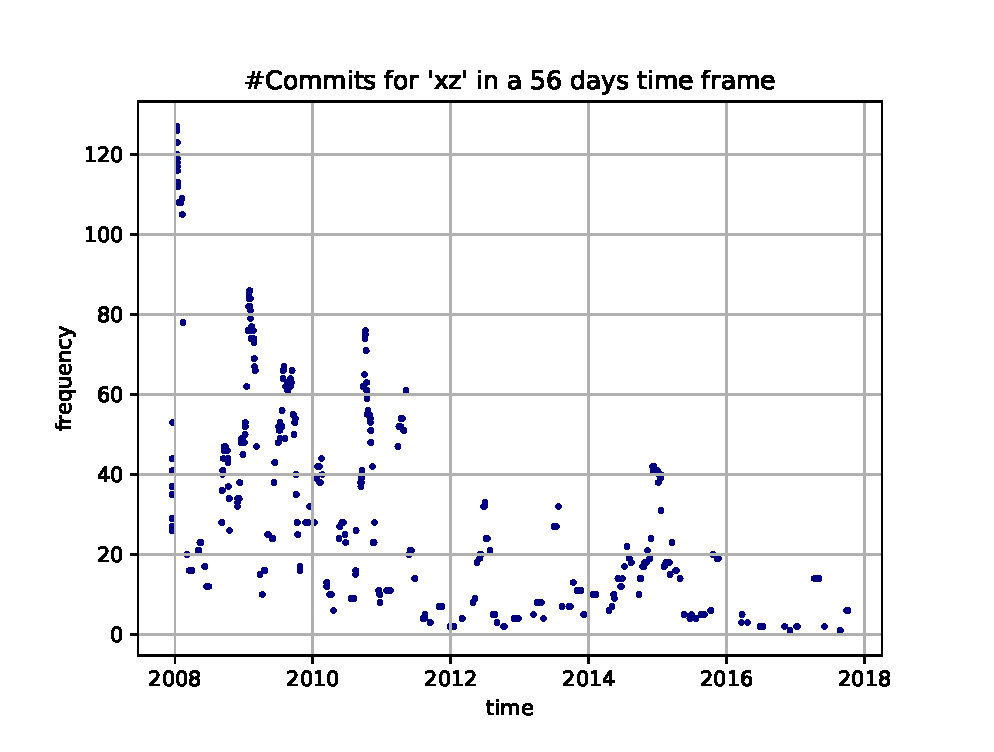
\includegraphics[width=0.4\textwidth]{images/activity_xz.eps}} 
%\subfloat[]{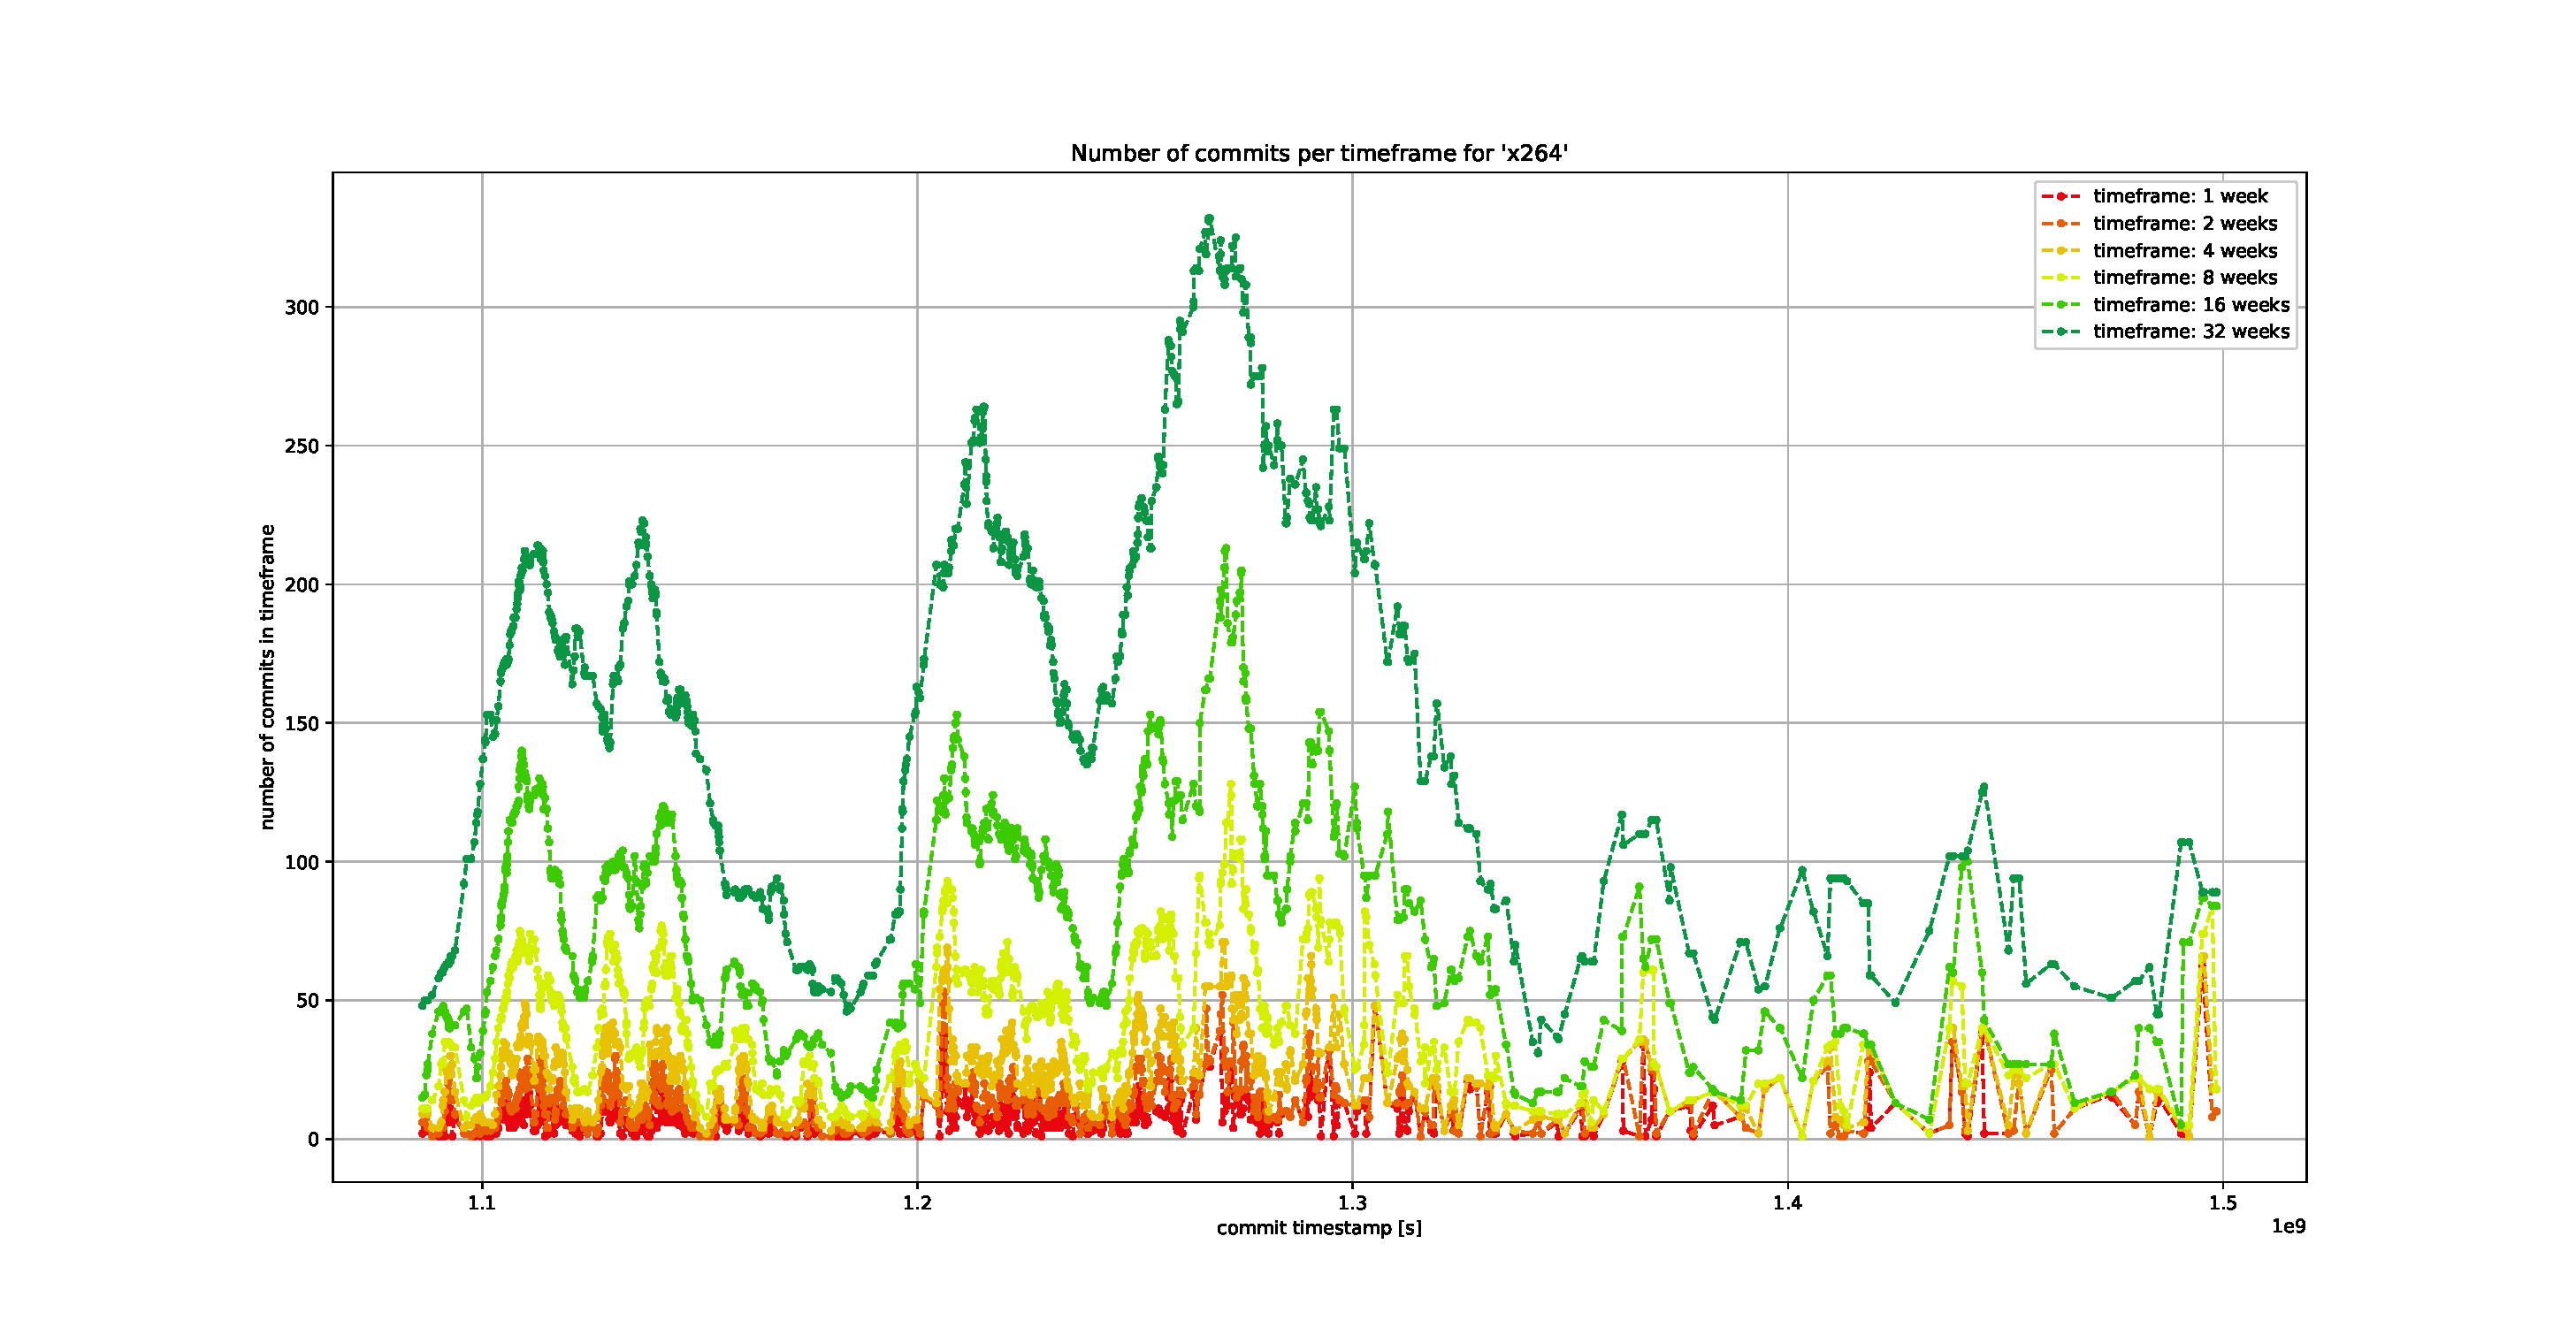
\includegraphics[width=0.4\textwidth]{images/activity_x264.eps}}
%\caption{Potential for 0.5 V bias.} 
%\label{fig:EcUND} 
%\end{figure} 

The assessment of performance evolution for a software system entails the
assessment of changes in performance measures over multiple versions of a
software system. To comprehend its version history, there exists a variety of
resources that can be employed, ranging from logs of a version control system
(VCS), such as Git, SVN, or CVS, over more elaborate documentations, such as
bug reports, to domain- or developer knowledge regarding the evolution of the
software system, such as requirement artifacts or mailing history. While VCS
logs usually record all fine-grained and iterative changes, bug reports or
release notes sketch larger chunks of the software evolution. Moreover, all
different resources focus on certain aspects of the software system’s
evolution, so that, for instance, VCS logs enable a developer-centered
perspective, whereas bug reports or release notes represent a more
user-centered perspective. That is, the assessment of performance for multiple
revisions of a software system always is placed in a certain context, such as
performance evolution of end-user versions when assessing releases only.

To understand how performance of a software system evolves in practice, it is
necessary to learn from which perspective we can observe and reenact
performance evolution for two reasons. \emph{First}, performance quality is a
concern which is omnipresent throughout development and usage of a software system.
Ideally, performance regressionis is avoided or handled during development, yet,
not least due to insufficient assessment, performance defects heavily
impact end-user satisfaction. \emph{Second}, we aim not to only understand
performance evolution, but to design tools leveraging this knowledge, for instance, to
predict performance for future changes, or to highlight performance-critical
code sections. For this purpose, efficient strategies to assess multiple
versions are inevitable.

Research so far has addressed the assessment of a software system’s revision
history under the umbrella of repository mining, for instance, to localize bugs
(Moin \& Khansari, 2010) or to XY. Nonetheless, so far there exists little to no
research addressing the question what perspective of version-related resources
as well as the choice of versions might reveal about performance evolution. The
task of selecting resources and a sample set of versions to analyze can be
conceived as a sampling strategy, where the objective is to cover interesting
entities (performance changes, in our case) while limiting the sample size to
keep the effort necessary reasonable. In this section, we develop and discuss
three sampling strategies to select versions from the overall version history.
These sampling strategies are subsequently applied to a selection of
configurable software systems and evaluated in the remainder of this thesis.


%\begin{figure}
%\def\tabularxcolumn#1{m{#1}}
%\begin{tabularx}{\linewidth}{@{}cXX@{}}
%\begin{tabular}{c}
%\subfloat[Activity Graph for \texttt{GNU XZ}, generated from 399 versions
%between March 24, 2017, and August 14, 2017. The earliest release version is
%\texttt{5.1.1alpha}, the latest is \texttt{5.3.0alpha}.]
%{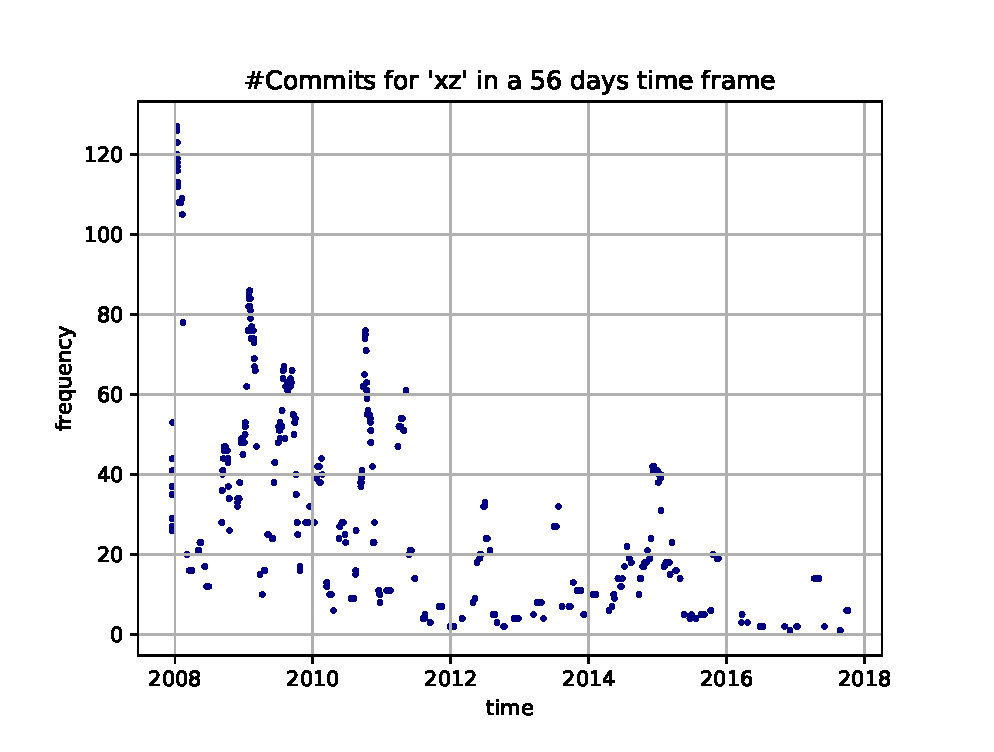
\includegraphics[width=0.99\textwidth]{images/activity_xz.eps}}
%\\
%\subfloat[Activity Graph for \texttt{x264}, generated from 2851 versions
%between June 3, 2004, and June 26, 2017. The earliest release version is
%\texttt{BUILD 1} from, the latest is \texttt{BUILD 149} from
%X.]{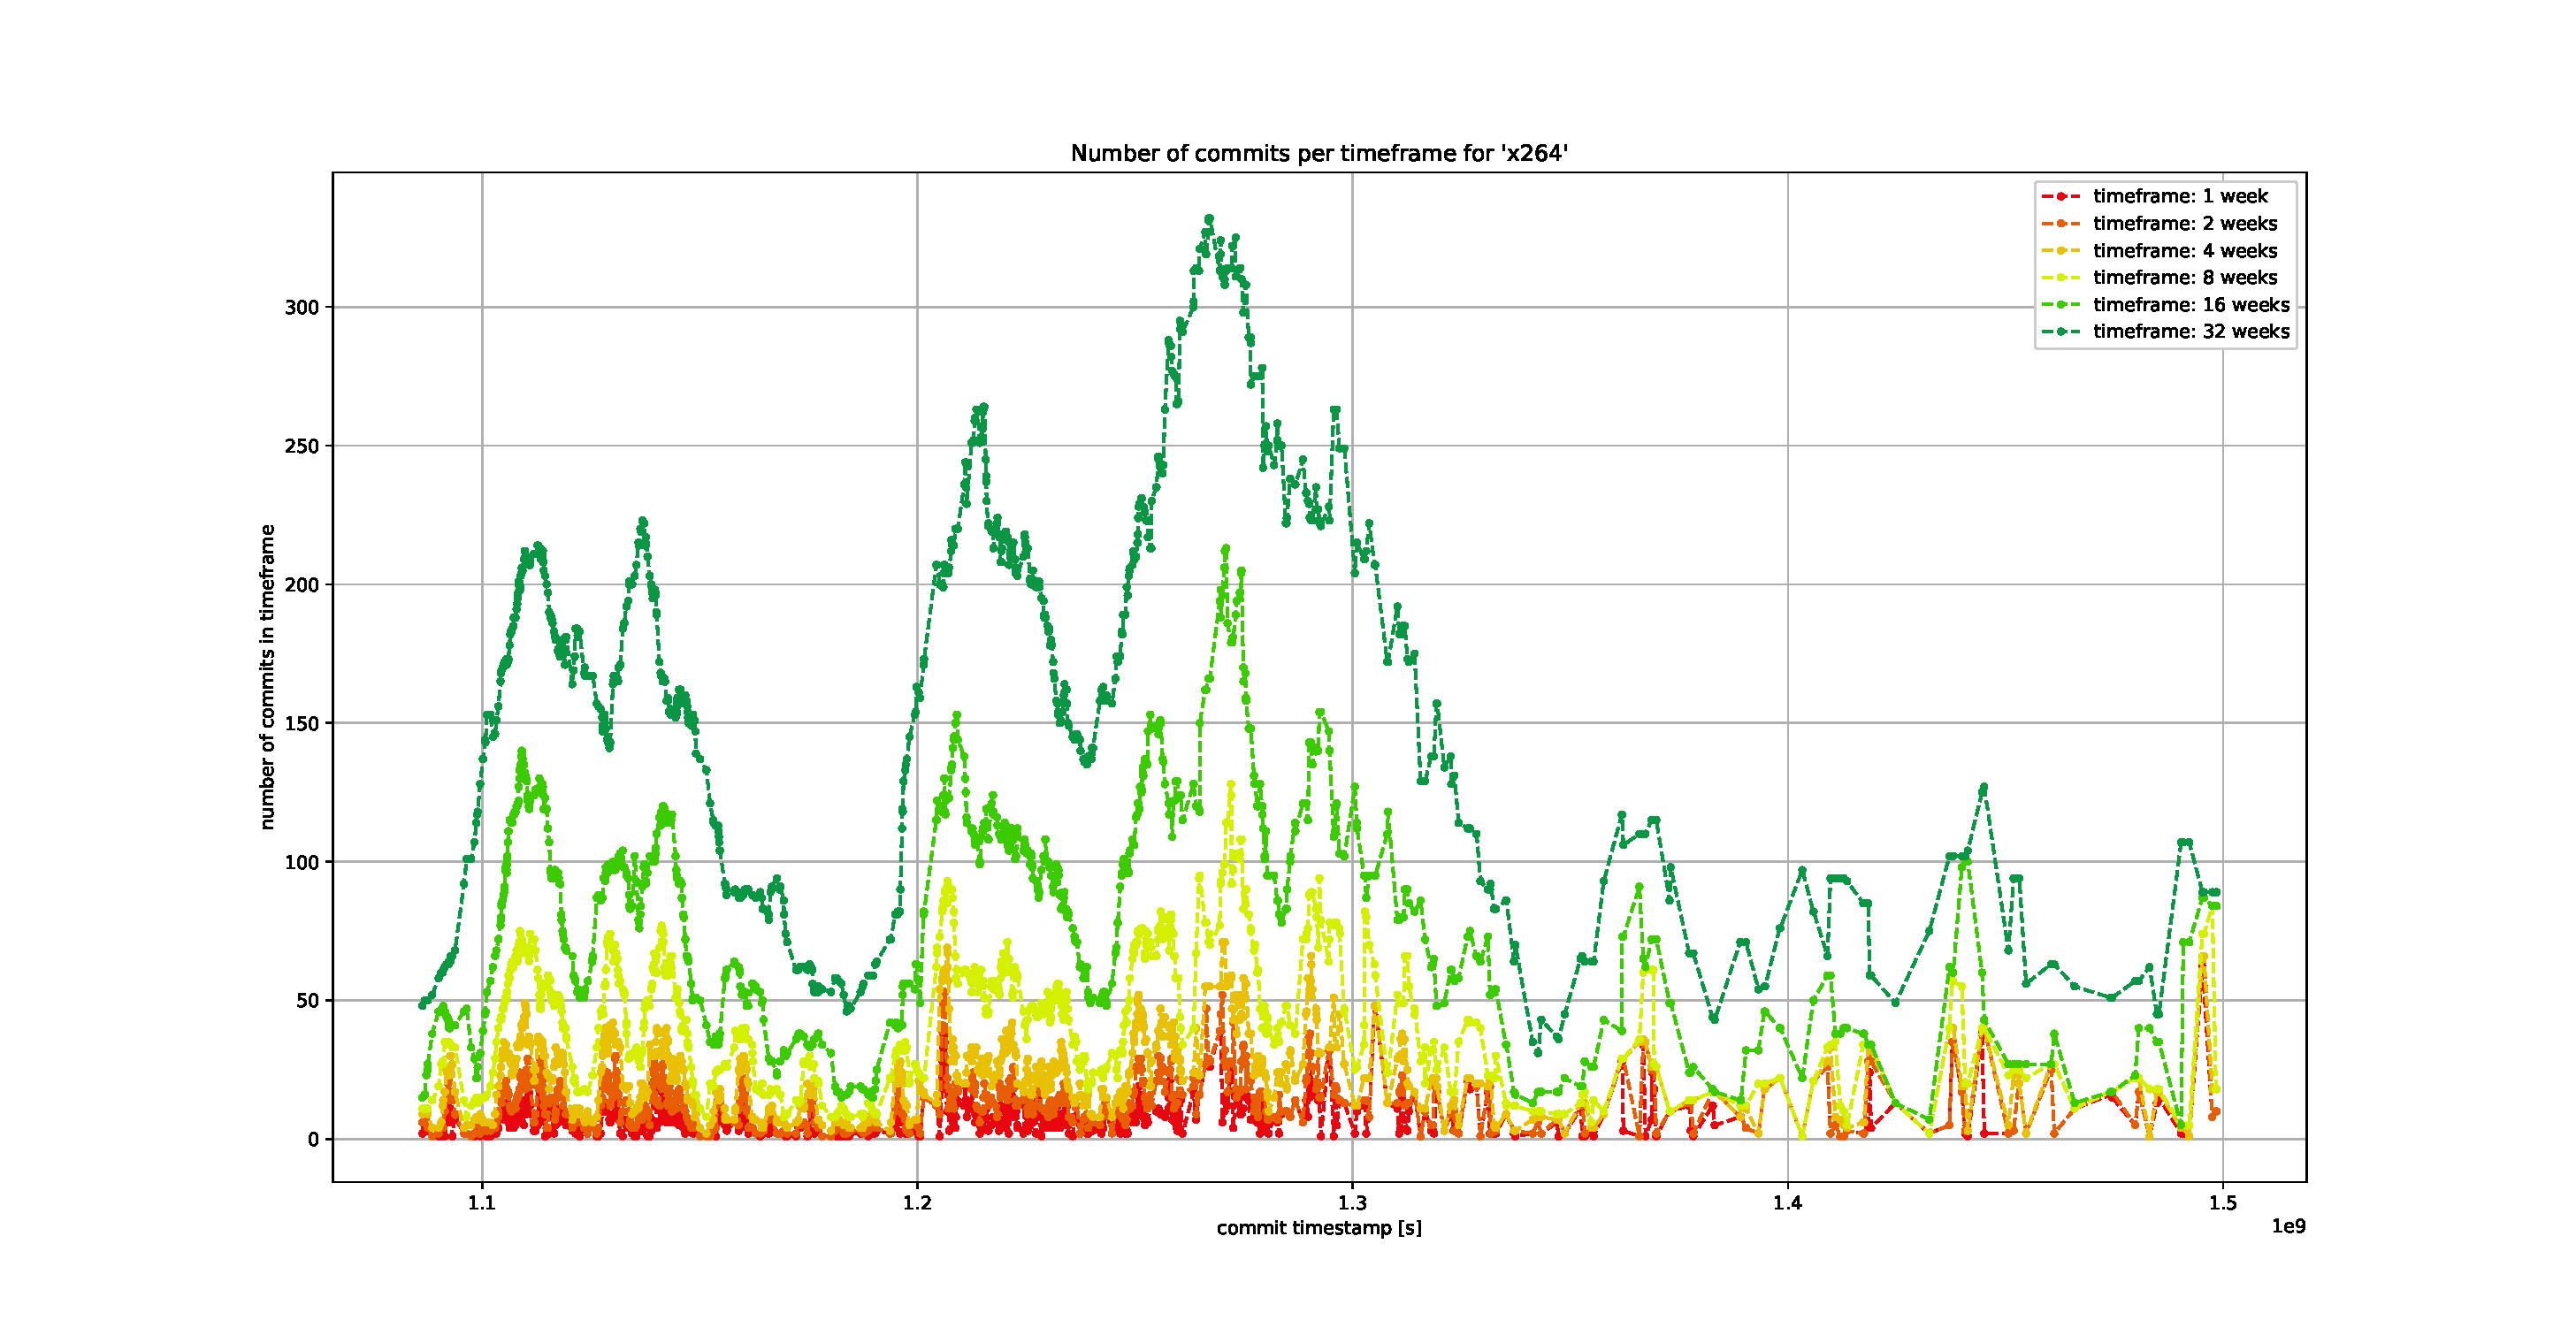
\includegraphics[width=0.99\textwidth]{images/activity_x264.eps}}\\
%\end{tabular}
%\end{tabularx}
%\caption{Commit activity for two sample systems, the compression
%utility \texttt{GNU XZ} and the video encoder \texttt{x264}. For each version,
%the activity is measured as the number of commits that were pushed within a
%certain timeframe after or before the actual commit. The timeframes range from
%one week to 32 weeks, as shown in the legendary.}
%\label{fig:ActivityGraphs}
%\end{figure}


\section{Remarks}
Before we dive into different approaches to select a sample set of revisions,
we need to define a general framework for evaluating a sample set of revisions
as well as respective revision sampling strategies with respect to performance
change history.

\paragraph{Revision Sample Sets.} The first question is, what criteria we take
as a basis for rating a sample of revisions as “meaningful”. First, our
intention is to obtain a representative description of a software system’s
performance change history while only assessing a fraction of revisions. That
is, assessing a representative sample of revisions should yield a performance
change history similar to the assessment of all revisions. Since we are
interested in revisions for which performance measurements change, these
revisions should be contained in a representative sample. Second., especially
in the context of variability, a performance change might only affect a subset
of the assessed configurations. A representative sample set, therefore, should
describe a history of significant performance changes with respect to all
variants assessed. We consider a performance change to be significant, if it
affects a significant portion of the sample of variants (\emph{effect range}),
and if the relative change in performance measurements is significantly huge
(\emph{effect magnitude}). While the former significance criterion can
unambiguously defined by a threshold number of variants, for the latter one one needs to define how
to summarize relative performance change among all variants. For instance, a
performance change may have a significant magnitude, if the average deviation
of performance measurements for all variants is greater than a specified
threshold value.

\paragraph{Revision Sampling Strategies.} The second question addresses the
rationale behind a revision sampling strategy. To obtain representative sample
sets, sampling strategies are intended to utilize knowledge about the total
volume to select sample sets from. For instance, pair-wise sampling aims to
cover most feature interactions. Similarly, we demand for a meaningful revision
sampling strategy to exhibit a certain rationale or coverage criterion. If we
conceive a sampling strategy as a binary classificator that, in our case,
decides whether in a revision a performance change is likely, or performance
measurements might have changed compared to prior commits, we want  this
classifier to be sensitive, i.e., to have a preferably high true positive rate.
That is, a sampling strategy is meaningful if we learn which revision features
most likely indicate performance evolution.



\section{Sampling Strategy Classification}
